\chapter{CEMicro Implementation}
\label{sec:impl}


\section{Setting up the Development Environment}

\begin{itemize}
  \item \done{Visual Studio Code (code editor) https://code.visualstudio.com/}
  \item \done{Git (version control) https://git-scm.com/}
  \item \done{Virtualisation with Docker}
  \item \done{Node.js}
  \item \done{Challenge: Setting up git/bash on windows}
  \item \done{Challenge: File permissions for docker on windows}
\end{itemize}

It seems trivial to treat the development environment in this chapter, but that would be a disservice to any programmer. The development environment is an essential part of writing an application and can be as much of a time sink as software bugs, as we will see. I am used to developing on a Mac operating system. Mac is based on Unix and offers a built-in Bash shell, basically just like any Linux machine, while Windows uses an entirely different foundation for its operating system. All the technologies which work with cloud computing and distributed services operate on Linux systems because the internet runs on Linux\footnote{Yeah, sorry Microsoft}. We are talking about technologies like Git version control, Docker container virtualization, and Node.js and its packet manager NPM. The machine Capgemini provided me with is a Windows computer.

I first set up Visual Studio Code, currently the most popular code editor, especially among web developers and developed by Microsoft ~\cite{stackoverflow.2019}. Next, I set up git\footnote{https://git-scm.com/downloads}, which comes with a complete Bash environment, howbeit with a reduced feature set. Bash stands for "Bourne Again Shell" and is a variation of the default Unix shell, a command-line interface. An average user usually never uses the command line but interacts with generated user interfaces (GUI) of a program. In a shell, the user can interact with programs by typing one-line commands. For example, \inlinecode{rm -rf test-dir/} instructs the simple 'remove' program to delete the 'test-dir' folder with all its content. This way of using programs is handy for programmers and system administrators in their work, especially if running commands on remote computers through SSH\footnote{Secure Shell, a way to use the shell of a remote computer} sessions.

\begin{figure}[ht]
  \centering
  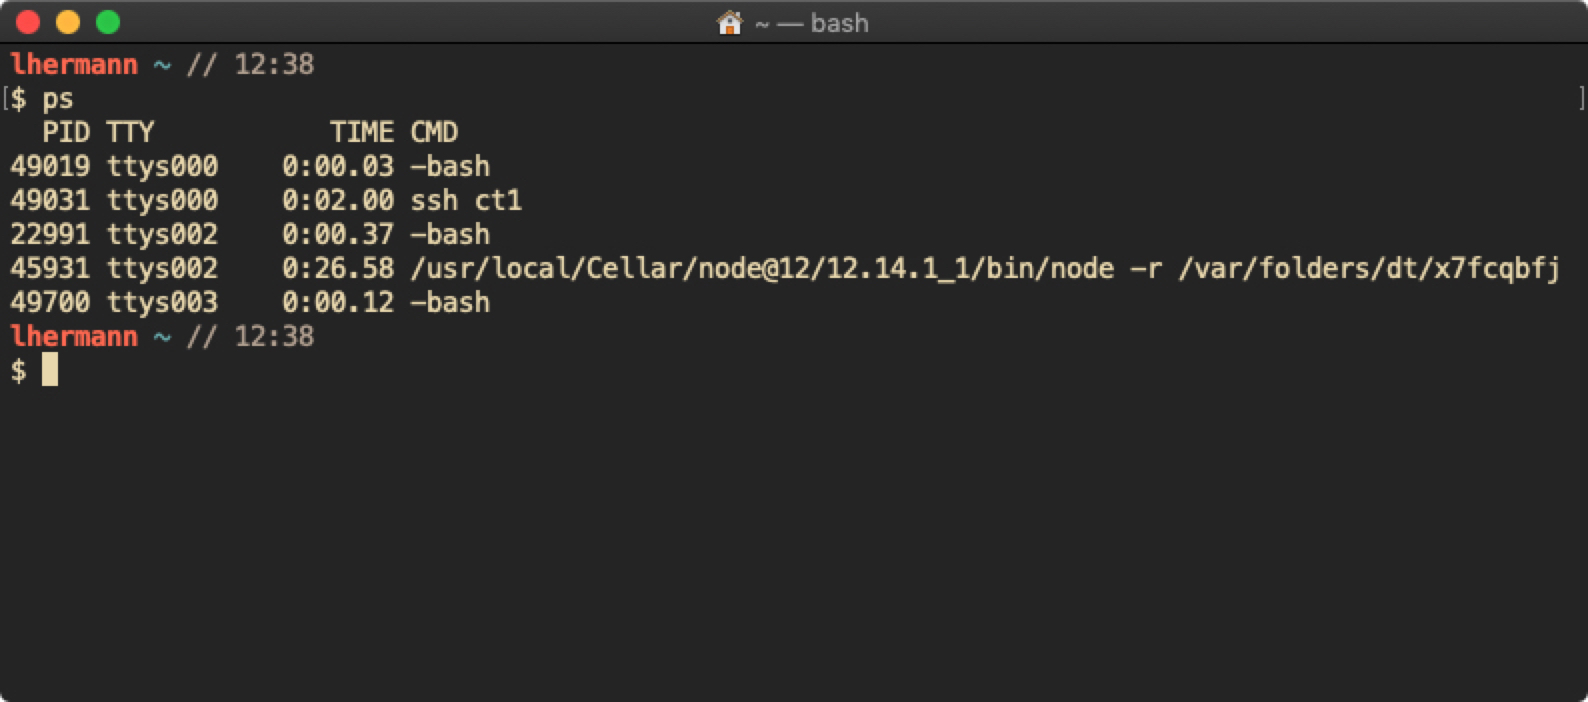
\includegraphics[width=0.75\linewidth]{assets/example-bash-window.jpg}
  \caption{Example for a bash terminal executing the 'ps' command}
\end{figure}

Because I planned to write the entire application in JavaScript, I set up a Node.js environment\footnote{https://nodejs.org/}. JavaScript is an interpreted language; it means that the code does not need to compile to machine code like Java, for example, but the Node runtime reads the JavaScript file and translates it for the computer on the fly. It means that I can start a program by simply typing \inlinecode{node main.js} into the shell, which then executes the contents of main.js. Furthermore, I can install a JavaScript tool like Nodemon\footnote{https://www.npmjs.com/package/nodemon} with \inlinecode{npm install nodemon} that watches the JS\footnote{JS is short for JavaScript} files on my systems and restarts the application whenever I change the file. This provides instant feedback, in the form of an updated application or error messages, and makes development comfortable.

\begin{figure}[ht]
  \centering
  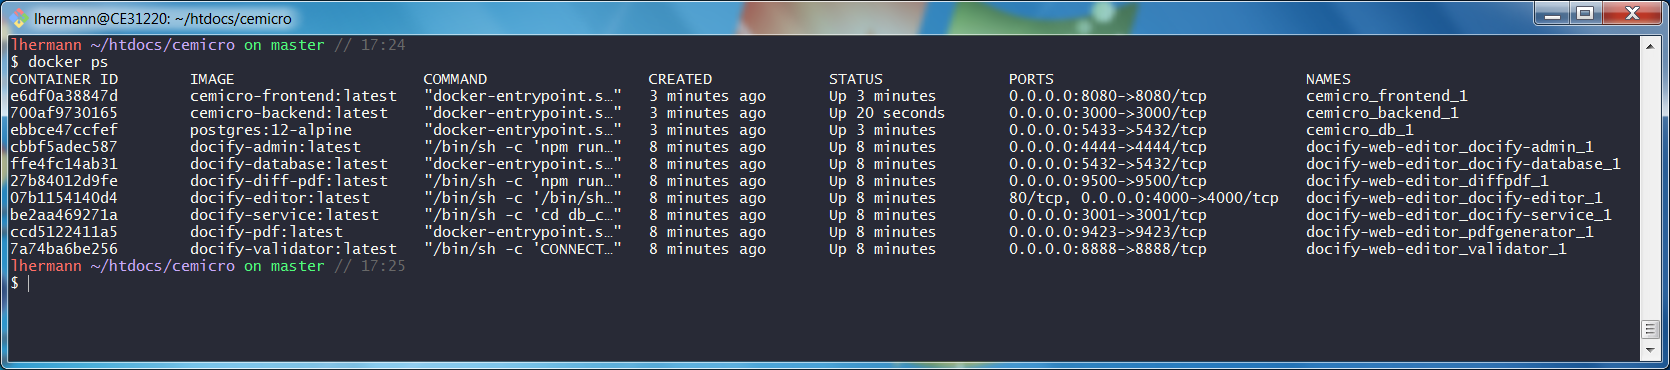
\includegraphics[width=1\linewidth]{assets/terminal-docker-ps.png}
  \caption{'docker ps' shows all running docker containers}
\end{figure}

Docker\footnote{https://www.docker.com} is a tool that can run the software in a container. A container is like an application that brings its entire ecosystem with it, howbeit a very simplified one, so that it doesn't become too large. This application then runs in isolation from anything else on the host system. This is very useful because it allows the developer to run dependencies like databases or other services for an application without the hassle of installing them on the system manually and the difficulty of handling different versions. For the development of CEMicro, I ran my PostgreSQL database in a docker container. I also needed a running instance of the Docify service, itself a combination of six containers, which I downloaded and started in Docker. The \inlinecode{docker-compose} command provides a very convenient way to start all required containers for an entire application at once. These containers then run in the background, and the developer can concentrate on his current code.

One challenge I faced with setting up bash on windows was the limited way in which the shell environment of the git application works. Familiar commands and shell setups on Unix machines were not available under the Windows environment, and it took me a while to work around this limitation. Another problem arose with Docker in that it works with Unix file system permissions. On a Unix system, every file has a set of nine permissions, read, write and execute separate for the user, the group and others\footnote{The details about Unix file permissions go beyond this chapter, for more info see https://www.tutorialspoint.com/unix/unix-file-permission.htm}, this system is part of the hard drive format and OS kernel\footnote{A kernel is the bottom-most layer of an operating system}. Windows does not have any file system permissions; it's not part of the operating system. Instead, Windows handles users and groups with dedicated services, and this is also the reason why there are so many more worms and viruses for Windows. The Docker environment for Windows fakes those permissions. But for specific requirements, for example, when using Docker volumes, these permissions need to be changed to work. It is possible to do this, but I couldn't find out how and I assume it has to do with a user management service, which is not accessible under the closed business setup of the machine Capgemini gave me. It, therefore, took me a while to find a workaround for Docker volumes so that they only exist within the virtual environment and don't come in contact with the Windows host.

\section{Application Programming Interface}
\label{sec:impl:api}

\begin{itemize}
  \item \done{REST}
  \item \done{Swagger/OpenApi}
  \item \done{Single source of truth}
  \item \done{Discarded: Saving Templates in CEMicro (see single source of truth page)}
  \item \done{Discarded: swagger-tools}
\end{itemize}

The CEMicro service deals with three different objects\footnote{In programming, an object is like a container for data} — the template, the configurable element, and its items. The template contains the template string in combination with sample data for the placeholders inside the template. The configurable element, as discussed in the section on page \pageref{sec:arch:understanding}, a holder for the individual properties as well as the name and the default value. And the configurable element item which is one individual set of the properties of table \ref{table:ce-properties}.

\begin{table}[!ht]
  \begin{center}
    \begin{tabular}{|l|l|l|}
      \hline
      Action & Route & Description \\
      \hline\hline
      GET & /templates & Get a list of template abstracts \\
      \hline
      GET & /templates/\{market\} & Get a list of template abstracts by market \\
      \hline
      GET & /templates/\{market\}/\{name\} & Get a template by market and name \\
      \hline
      GET & /templates/\{market\}/\{name\}/pdf & Get the PDF of a template by market and name \\
      \hline
      GET & /configurable-elements & Get a list of Elements for the given parameters \\
      \hline
      GET & /configurable-elements/\{id\} & Get an Elements by id \\
      \hline
      PATCH & /configurable-elements/\{id\} & Update an Element by id \\
      \hline
      GET & /configurable-elements/\{id\}/items & Get all Items for an Element \\
      \hline
      POST & /configurable-elements/\{id\}/items & Create an Item for an Element \\
      \hline
      GET & /configurable-element-items/\{id\} & Get an ElementItem by id \\
      \hline
      PUT & /configurable-element-items/\{id\} & Update an ElementItem by id \\
      \hline
      PATCH & /configurable-element-items/\{id\} & Patch an ElementItem by id \\
      \hline
      DELETE & /configurable-element-items/\{id\} & Delete an ElementItem by id \\
      \hline
    \end{tabular}
  \end{center}
  \caption{API endpoints of the CEMicro backend}
  \label{table:api-endpoints}
\end{table}

Table \ref{table:api-endpoints} shows all the API endpoints of CEMicro. We can see that a market-name tuple uniquely identifies a template. That means a template name itself is not unique because two markets, like the Netherlands and France, can use the same template name. To make sure these templates do not get mixed up, they are namespaced by the market. Also, observe that there is no POST or PUT actions for templates, that's because templates are not saved in the CEMicro database but fetched from the Docify service whenever requesting this endpoint.

One important concept is the single source of truth, meaning that one piece of information only exists in one place. This is especially important when working with microservices and other concepts of distributed architectures. Since the services and thus the programming logic is distributed, information, by necessity, also needs to be distributed. However, as just established, we do not want duplication of information. Thus, with microservice architectures, one piece of information should only exist inside a single microservice. CEMicro solves this the single source of truth principle by requesting templates on the fly from the Docify service and only saving configurable elements and their items in its database.

Initially, I planned to include templates in the database because it is such an essential part of the application. The frontend needs to list all the available templates, and configurable elements are essentially placeholders within the template. However, saving the templates in our database would mean duplication of the information because Docify handles them. It would be possible for docify to send a notification to CEMicro whenever a template changes, but the easier way is to fetch templates fresh every time we need them.

Both elements and element items are saved in the CEMicro database and entirely managed by it. It is common to provide CRUD actions for every resource. CRUD stands for CREATE-READ-UPDATE-DELETE, the four principal actions for data. In the table, we can see that element items have all four CRUD operations plus PATCH, which is a partial update function where only a subset of properties has to be provided. Configurable elements, however, do not have four CRUD operations. That's because I decided to create them on the fly. Whenever the user opens a template in the frontend, it requests all the elements from the backend. At that point, the backend parses the template string for a list of all the necessary configurable elements. It then compares this list with the database and creates an element that is missing before returning the complete list of elements to the frontend. This way, the user is saved the hassle of manually creating an element after adding it to the template in Docify. It saved one working step. However, during the debriefing with the project manager, we concluded that it would be better to additionally offer the manual option to the user so he can create and delete elements as needed.

\begin{figure}
  \centering
  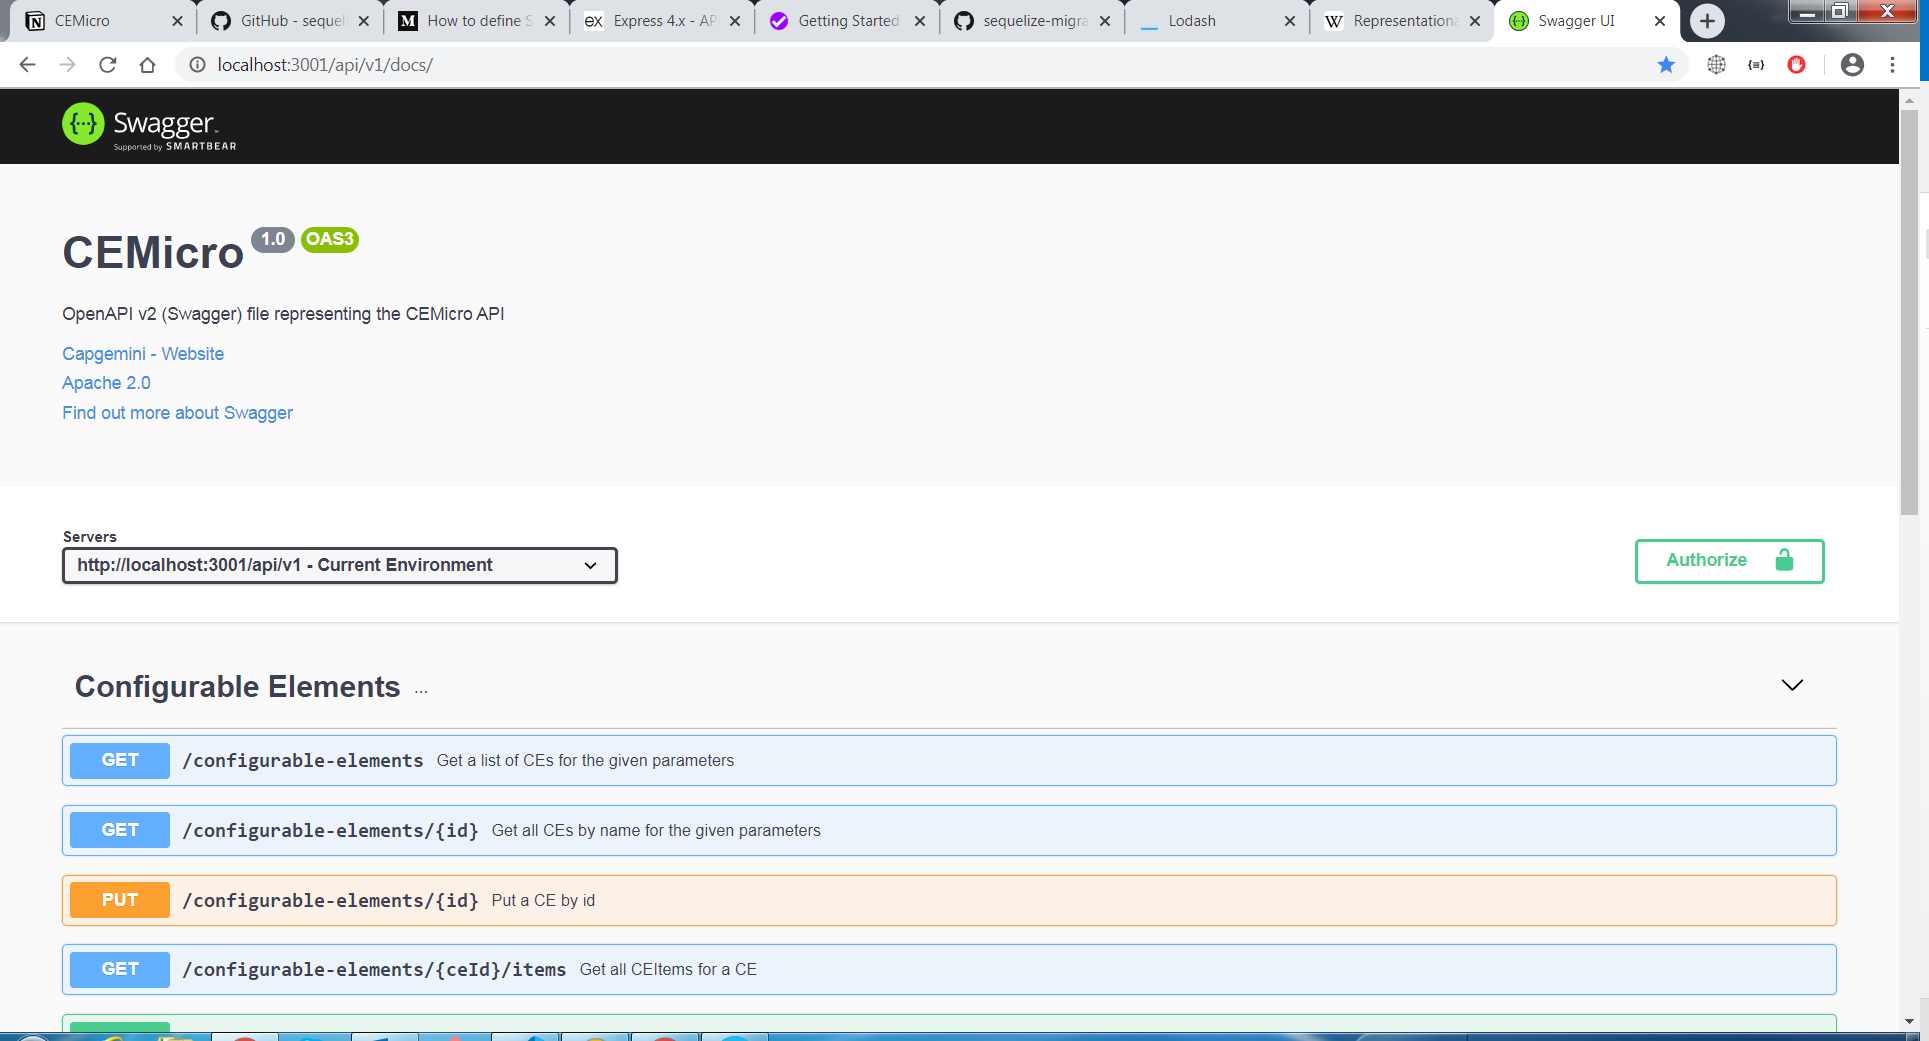
\includegraphics[width=0.8\linewidth]{assets/swagger-api-docs.png}
  \caption{Interactive API documentation with Swagger}
  \label{fig:api-docs}
\end{figure}

The appendix, page \ref{sec:appendix}, shows an excerpt of the \inlinecode{openapi.yml} file. This file is the authoritative documentation for the API. Swagger\footnote{https://swagger.io}, the open-source project behind the OpenAPI standard, provides tools to generate an interactive documentation page from this file automatically, see figure \ref{fig:api-docs}. Docify uses a library called "swagger-tools" to automatically generate some scaffolding for their code directly from their OpenAPI file. This approach saves some repetitive coding and helps to tie the functional code and the documentation together. For CEMicro, however, I decided to omit this library and add everything by hand because the project is stale, it didn't see any updates for two years, and does not support the latest version of the OpenAPI specification\footnote{See https://www.npmjs.com/package/swagger-tools}.


\section{Backend Framework with Express.js}

\begin{itemize}
  \item \todo{Tool: Nodemon}
  \item \todo{Tool: Express}
  \item \todo{Tool: Express Validator}
  \item \todo{MVC -> MVCS (Model View Controller Service)}
\end{itemize}


\section{Data persistance with PosgreSQL}

\begin{itemize}
  \item \todo{Sequelize https://github.com/sequelize/express-example}
  \item \todo{Discarded: Flyway-db, Umzug}
  \item \todo{Migrations: Sequelize}
\end{itemize}


\section{Frontend Framework with Vue.js}

\begin{itemize}
  \item \todo{To do ...}
\end{itemize}


\section{Virtualisation with Docker}

\begin{itemize}
 \item \todo{install packages, build, prune packages}
 \item \todo{...}
\end{itemize}


\section{Interfacing with the monolith development team}

\begin{itemize}
  \item \todo{Changes to Docify}
\end{itemize}


\section{Challanges during development}

\begin{itemize}
  \item \todo{Knowing how to set up the development environment}
  \item \todo{Understanding the task, see [CE Properties]
  \item \todo{Setting up git/bash on windows}
  \item \todo{File permissions for docker on windows
\end{itemize}

https://medium.com/@akash1233/change-file-permissions-when-working-with-git-repos-on-windows-ea22e34d5cee

https://www.notion.so/CE-Properties-7bf08f28c69344c1957e7072c1101fd6


\section{Documentation of CEMicro}

\begin{itemize}
  \item \todo{Providing a foundation for others to build on (Confluence, Readme, Thesis)}
\end{itemize}
